\documentclass[conference]{IEEEtran}

\usepackage[numbers]{natbib}
\usepackage{pgfplots}
\usepackage{amsmath,amssymb,amsfonts}
\usepackage{algorithmic}
\usepackage{graphicx}
\usepackage{textcomp}
\usepackage{xcolor}
\usepackage{pgf-pie}  
\usepackage{hyperref}
\usepackage{tikz}
\usepackage{multirow}
\usepackage{pgfplots}
\pgfplotsset{compat=1.18}
\usepackage[acronym]{glossaries}

\hypersetup{
    colorlinks=true,
    allcolors=.,
    urlcolor=blue}

\begin{document}

\newcommand{\authcite}[1]{\citeauthor{#1} \cite{#1}}

\title{A systematic review on produce defect detection and quality assessment using artificial intelligence}

\author{
    \IEEEauthorblockN{1\textsuperscript{st} João Silva}
    \IEEEauthorblockA{\textit{Departamento de Engenharia Informática} \\
    \textit{Instituto de Superior de Engenharia do Porto} \\
    1150425@isep.ipp.pt}
    \\
    \IEEEauthorblockN{3\textsuperscript{th} Nuno Costa}
    \IEEEauthorblockA{\textit{Departamento de Engenharia Informática} \\
    \textit{Instituto de Superior de Engenharia do Porto} \\
    1171584@isep.ipp.pt}
    \\
    \IEEEauthorblockN{5\textsuperscript{th} Diogo Formosinho}
    \IEEEauthorblockA{\textit{Departamento de Engenharia Informática} \\
    \textit{Instituto de Superior de Engenharia do Porto} \\
    1210056@isep.ipp.pt}
    \and
    \IEEEauthorblockN{2\textsuperscript{nd} João Santos}
    \IEEEauthorblockA{\textit{Departamento de Engenharia Informática} \\
    \textit{Instituto de Superior de Engenharia do Porto} \\
    1161023@isep.ipp.pt}
    \\
    \IEEEauthorblockN{4\textsuperscript{th} José Araújo}
    \IEEEauthorblockA{\textit{Departamento de Engenharia Informática} \\
    \textit{Instituto de Superior de Engenharia do Porto} \\
    1180943@isep.ipp.pt}
    \\
    \IEEEauthorblockN{6\textsuperscript{th} Francisco Cabrita}
    \IEEEauthorblockA{\textit{Departamento de Engenharia Informática} \\
    \textit{Instituto de Superior de Engenharia do Porto} \\
    1210058@isep.ipp.pt}
}
\maketitle

\begin{abstract}

The Food and Agriculture Organization of the United Nations indicates that the gross production value of produce across the world in 2020 reached over 4.145 trillion US dollars. With such large-scale production, transportation required to deliver these foods to consumers. With this, the post-harvest process has become crucial to reduce waste, preserve said foods and provide the end consumer with fresh, quality items. Additionally, regulated markets usually include minimum requirements on produce quality and appearance. With the automation of post harvest processes in the agricultural sector, systems are and have been designed to detect, grade and sort fruit and vegetables in a production line environment. This systematic review presents three research questions aimed at providing an overview of state of the art produce quality assessment and defect presence artificial intelligence based systems. The results have shown a great variety of produce target types, detection methods and techniques, objective metrics and artificial intelligence techniques used. The results of this review are also relevant for devising new systems that target untargeted produce types and unresearched detection systems.

\end{abstract}

\begin{IEEEkeywords}
Artificial Intelligence, Produce, Fruits, Vegetables, Quality Assessment, Defect Presence, Review
\end{IEEEkeywords}

\section{Introduction}
\label{sec:intro}

Agriculture is one of the most important economic activities, sustaining livelihoods by securing food production and providing income \cite{FDES-1}, with a global gross value of 4.145 trillion US dollars in 2020 \cite{FAO1}. This sector has and continues to undergo a process of steady industrialization, through the increase of commercial farm size, commodity specialization and increase capital availability, among other factors \cite{10.2307/1243439}. This industrialization has caused an explosive increase in productivity for nearly all agricultural activity \cite{owidagriculturalproduction}. In order to take full advantage of this increased productivity, improvements are also required in the infrastructure and post harvest processes of a given agricultural unit, before the produce reaches the final consumer \cite{Food_and_Agriculture_Organization_of_the_United_Nations2010-hb}. With this, the post-harvest process has become crucial to reduce waste, preserve said foods and provide the end consumer with fresh, quality items \cite{foods6010008}. The previously mentioned improvements have materialized into facilities in which the produce can be stored, cleaned, prepared, sorted and packaged. However, with the large throughput of produce being processed in the aforementioned facilities, there is a need for systems that effectively monitor and sort said produce, taking into account defects and overall quality \cite{Mahalik2009}.

Furthermore, markets are usually regulated to include minimum requirements on produce quality and appearance, such as European Commission Implementing Regulation (EU) 543/2011, which sets out minimum quality requirements for a variety of produce, such as intactness, soundness and cleanliness \cite{eu-5432011}. In order to abide by the aforementioned regulation, producers must consider travel time and the possibility of spoilage within that time frame \cite{biv081}. Small defects in produce expand over time and can potentially spoil the whole item (be it a single produce item or a packaged set of items). Detection systems are already in place in post harvesting processes in the horticultural sector, identifying pathological, mechanical, physiological and internal defects \cite{Nturambirwe2020}.

The purpose of this work is to understand what factors can be monitored to ascertain the quality or defect presence in produce, what techniques and technologies are available to analyse and monitor produce in a industrial environment and how is artificial intelligence and related fields enhancing the usage of said technologies. To do this, three research questions are presented, and existing studies that may answer these questions are analysed and discussed in order to reach an overview of the current state of the art in the topics of produce quality analysis and defect detection using artificial intelligence, the evolution of the domain and their application in the post-harvest processing field.

The remainder of this document is structured in 4 sections:
\begin{itemize}
	\item Section \ref{sec:meth}, in which the procedure taken in this systematic review is presented in detail and all steps of the process are accounted for. In this section, we go from the definition of the research questions to the selection of the works to be included in this review, while explicating the inclusion and exclusion criteria and the data sources considered.
	\item Section \ref{sec:res}, in which we show which answers to the different research questions are proposed by the analysed studies to the best of our knowledge.
	\item Section \ref{sec:disc}, in which we take a deeper look at these studies and identify potential challenges and future directions for research.
	\item Section \ref{sec:conc}, which outlines the Conclusions and Future Work.
\end{itemize}

\section{Method}
\label{sec:meth}

The literature review will focus on the analysis of existing detection systems for the aforementioned situations, in order to assess how they answer to the research questions and how, if any, artificial intelligence is implemented in these systems. Analysing the challenges these systems face will allow us to establish how, and if, artificial intelligence can improve on existing systems and overcome the challenges set forth previously. Furthermore, the application context of this work lies in the field of artificial intelligence in detection systems in food processing operations and therefore existing works in this area will also be explored.
The goal of a systematic review of the literature is to extract, analyse and interpret a corpus of work pertaining to a specific field of study. Systematic reviews are meant to be through and to follow a sequential, detailed, specific and repeatable workflow that allows other researchers to achieve similar results. The methodology described by Kitchenham \cite{kitch} proposes that systematic reviews should follow a number of steps:
\begin{itemize}
	\item Development of the review protocol (including rationale and research questions);
	\item Processing;
	\item Analysis;
	\item Demonstration of the research's results;
\end{itemize}
With this such, this review starts by presenting the Research Questions and the motivating problem. Then, the data sources selected for this review will be presented, along with the process of selecting and using the most adequate combination of search terms that generated a query that could be equally used in the different data sources. Inclusion and Exclusion criteria, along with quality assessment criteria are described. Finally, a detailed account of the data extraction process is given, showing how the articles found in those data sources were continuously filtered until the final number of articles to review is reached.

\subsection{Research Questions}

For the purpose of this systematic review, we define the main research question as: ``What are the current applications of artificial intelligence based detection systems in the post harvest quality assurance processes?''. In order to properly answer this question, we can divide the main question into three more focused questions, which can be found in Table~\ref{tab:resquest}. The first question is mainly concerned with the physical factors that affect the quality analysis and defect detection processes. The second question then concerns itself with researching existing systems that utilize the aforementioned factors to detect defects and analyse the quality of produce. Finally, the last question focuses on identifying on which of these available systems integrate artificial intelligence, and to what degree this integrations provides usefulness to the overall system.

\begin{table*}
    \caption{Research Questions}
    \label{tab:resquest}

    \begin{tabular}{ll}
    \hline
        & \textbf{Research Question} \\
    \hline
        RQ1 & What objectives can be defined in the context of quality assessment or defect presence in produce? \\
        RQ2 &  What techniques and technologies are available to analyse and monitor produce in a industrial environment?\\
        RQ3 & What techniques and technologies previously researched utilize artificial intelligence, and how? \\
    \hline
    \end{tabular}
\end{table*}

\subsection{Data Sources}

The first step in the systemic review process is to identify the used data sources. It is advisable
to maintain a small number of comprehensible data sources, in order to maintain clarity and rigour \cite{Par2015}. Table~\ref{tab:edata} identifies the electronic databases chosen for this study. Within these data sources exist a degree of overlap, which will be accounted for in a following step.

\begin{table*}
    \caption{Electronic databases}
    \label{tab:edata}

    \begin{tabular}{lll}
    \hline
        Identifier & Database & URL \\
    \hline
        DS1 & ACM Digital Library & \url{https://dl.acm.org/} \\
        DS2 & IEEE Explore & \url{https://ieeexplore.ieee.org/} \\
    \hline

    \hline
    \end{tabular}
\end{table*}

\subsection{Search Terms}

Considering the application field of this research, along with the aforementioned questions, a number of domains were selected to assess not only how many studies have been performed, but how their combination affects the number of results. With this, consider the following domain selection and keywords, per Table~\ref{tab:resdom}.

\begin{table*}
	\caption{Domains and keywords used to select search terms}
	\label{tab:resdom}

	\begin{tabular}{ll}
	\hline
		Domain & Keywords \\
	\hline
		Artificial Intelligence & (``Artificial Intelligence'' OR ``Machine Learning'') \\
		Produce & (``Fruits'' OR ``Vegetables'' OR ``Berries'') \\
		Quality, Defects & (``Quality'' OR ``Defect'') \\
		Detection, Sorting & (``Classification'' OR ``Detection'' OR ``Grading'' OR ``Sorting'') \\
	\hline
	\end{tabular}
\end{table*}

Search terms were applied to Title, Abstract and Keywords. Different combinations of these domains were attempted and evaluated until a final search query was reached. Refer to Table~\ref{tab:resres} for the results of these attempts.

\begin{table*}[]
\caption{Combination of domains and respective results}
\label{tab:resres}
\begin{tabular}{llll}
\hline
\multirow{2}{*}{Domains}            & \multicolumn{3}{l}{Results} \\ \cline{2-4} 
                                    & ACM     & IEEE    & Total   \\ \hline
Artificial Intelligence             & 122,298 & 420,518 & 542,816 \\
Produce                             & 492,658 & 7,183   & 499,841 \\
Quality, Defects                    & 231,926 & 466,142 & 698,068 \\
Detection, Sorting                  & 246,506 & 747,608 & 994,114 \\
Artificial Intelligence AND Produce & 892     & 926     & 1,818   \\
Produce AND Quality, Defects        & 1,847   & 1,271   & 3,118   \\
Produce AND Quality, Defects AND Detection, Sorting                             & 1004 & 557 & 1,561 \\
Artificial Intelligence AND Produce AND Quality, Defects AND Detection, Sorting & 379  & 189 & 568   \\ \hline
\end{tabular}
\end{table*}

As can be inferred from Table~\ref{tab:resres}, we see that each individual domain provides a large volume of results. As such, the intersection of all domains provides us with a sufficient number of results that are more focused than other intersections, with some but no all defined domains. The final used query is as follows:

\begin{quote}
 (``Artificial Intelligence'' OR ``Machine Learning'') AND (``Fruits'' OR ``Vegetables'' OR ``Berries'') AND (``Quality'' OR ``Defect'') AND (``Classification'' OR ``Detection'' OR ``Grading'' OR ``Sorting'')
\end{quote}

\subsection{Quality assessment: inclusion and exclusion criteria}

In order to assess if a specific article should be included in this review, a set of rules were devised. These will evaluate a number of parameters unrelated to the actual content of the article (e.g. peer-review status, release format, article quality and relevance). Table~\ref{tab:inccrit} and Table~\ref{tab:exccrit} showcase the inclusion and exclusion criteria used, respectively.

\begin{table*}
	\caption{Inclusion Criteria}
	\label{tab:inccrit}

	\begin{tabular}{ll}
	\hline
		 & Inclusion Criteria \\
	\hline
		IC1 & The source belongs to the field of agricultural/food engineering  \\
		IC2 & The source describes a novel contribution to the fields of study \\
		IC3 & The source describes a methodology or system for produce quality control or defect detection, including novel sensor and software components \\
		IC4 & The source describes what factors are being measured in order to obtain the results described \\
	\hline
	\end{tabular}
\end{table*}

\begin{table*}
	\caption{Exclusion Criteria}
	\label{tab:exccrit}

	\begin{tabular}{ll}
	\hline
		 & Exclusion Criteria \\
	\hline
		EC1 & The source is over 5 years old \\
		EC2 & The source is a systematic review \\
		EC3 & The source is not written in English \\
		EC4 & The contribution to the fields of agricultural/food engineering and artificial intelligence is not clear of not the focus of the source \\
		EC5 & The source does not provide sufficient information on the specifications of the techniques, methodologies or systems used or developed \\
	\hline
	\end{tabular}
\end{table*}

\subsection{Data Extraction}

Figure~\ref{fig:elig} represents the process used to undertake this systematic review.

\begin{figure*}[tb]
	\centering
	\includegraphics[width=0.45\textwidth]{images/eligibilityprocess.png}
	\caption{Eligibility Process Flow Diagram}
	\label{fig:elig}
\end{figure*}

The process of data extraction begins with extracting data from the pre-defined digital libraries by applying the aforementioned search terms and filtering the data entries by the last five years of studies (a time interval from 2017 to 2022). This timetable was selected by taking into consideration available working hours from the authors of this document, as well as maintaining a reasonable both new research and foundational research. The search brought forth 366 papers to review.
The following step was to remove duplicates. Of the initial 366 papers, 7 were duplicates, in accordance to title, abstract and DOI number filter search. As per \authcite{kitch}, of these duplicates the most recent release was included in the process.
The resulting 352 papers moved on to the next stage of the process, screening. In this, the papers were subject to sequential screening: abstract screening, relevance reassessment and full-text screening.
The first step, abstract screening, evaluates papers based on their abstract, ascertaining from that their relevance to the systemic review topics. In this stage, 208 papers were deemed irrelevant to the research at hand, with 58 papers considered relevant and 48 papers requiring further analysis to determine their relevancy.
In the next step, the relevance reassessment, the papers deemed possibly relevant are subject to a quick read through in order to determine their relevancy. Of the 48 papers that required reassessment, 28 were classified as relevant and 20 were deemed irrelevant.
In the final step of screening, the full text screening, a further 23 papers were removed from this review, on the basis of purview. We are left with 63 papers at the end of the screening stage.
At the eligibility stage, the papers are thoroughly read in order to understand what their contributions to the fields at hand. As such, from the 63 papers, 38 are included in this review.

\section{Results}
\label{sec:res}

This section describes the results obtained in this systematic review, with a particular focus on answering the question defined in Table~\ref{tab:resquest}. All of the papers in this review were specific on the type of produce their research targeted, information which is specified in Table~\ref{tab:restype}.


\begin{table*}
\caption{Produce Type in produce defect detection and quality assessment papers}
\label{tab:restype}
\begin{tabular}{p{0.85\textwidth}l}
\hline
Paper                 & Produce Type     \\
\hline
\authcite{Pande2019-fz}, \authcite{Nie2019-hx}, \authcite{Hamza2018-sc}, \authcite{Muladi2019-jp}, \authcite{Stasenko2021-jt}, \authcite{Zhang2020}, \authcite{Kumar2021}, \authcite{Zeb2022}, \authcite{Tran2021}, \authcite{Geng2021} &
  Apple \\
\authcite{Zeb2022}                                                & Apricot       \\
\authcite{Saragih2021-wu}, \authcite{Mishra2022-kz}, \authcite{Al_Haque2021-fw}, \authcite{Kumar2021} &
  Banana \\
\authcite{Hasan2021}                                              & Bitter Gourd  \\
\authcite{Park2021-de}, \authcite{Annaland2020}                   & Cherry        \\
\authcite{Fadchar2020-pp}                                         & Coconut       \\
\authcite{EAngelia2021}                                           & Coffee Bean   \\
\authcite{Anita2020-nm}, \authcite{Tamayo-Monsalve2022-ud}        & Coffee Cherry \\
\authcite{Castro2019-hk}                                          & Gooseberry    \\
\authcite{Zeb2022}                                                & Grapes        \\
\authcite{Kumar2021}                                              & Guava         \\
\authcite{Pande2019-fz}                                           & Lemon         \\
\authcite{Kumar2021}                                              & Lime          \\
\authcite{Zeb2022}                                                & Loquat        \\
\authcite{Prabhu2022-zh}, \authcite{Vo2019}, \authcite{Basri2018}, \authcite{Pise2018}, \authcite{Wagimin2022}, \authcite{Zeb2022}, \authcite{Bhole2020} &
  Mango \\
\authcite{Mohtar2019-ru}, \authcite{Azizah2017}                   & Mangosteen    \\
\authcite{Zeb2022}, \authcite{Rangel2021}                         & Melon         \\
\authcite{MiraeiAshtiani2021}                                     & Mulberry      \\
\authcite{Nipas2022}                                              & Onion         \\
\authcite{Pande2019-fz}, \authcite{Kumar2021}, \authcite{Zeb2022} & Orange        \\
\authcite{GarillosManliguez2021}                                  & Papaya        \\
\authcite{Choi2018-xp}, \authcite{Pande2019-fz}                   & Pear          \\
\authcite{Lu2018}                                                 & Pear          \\
\authcite{Basri2018}                                              & Pitaya        \\
\authcite{Zeb2022}                                                & Plum          \\
\authcite{Kumar2021}                                              & Pomegranate   \\
\authcite{Indrabayu2019}                                          & Strawberry    \\
\authcite{Bautista2020-ye}, \authcite{Shi2019}                    & Tomato     \\

\hline
\end{tabular}
\end{table*}


\subsection{RQ1 - What objectives can be defined in the context of quality assessment or defect presence in produce?}

Of the retrieved papers, a large majority (19) focuses on the quality and presence of defects in the analysed produce as a measurable goal of their research. As quality is extremely connected to defects and defect presence is a step in quality assessment in some of the papers reviewed, both of these were considered to be a single instance of an objective. Some papers also defined quality exactly as the non-existence of defects in the produce. Furthermore ripeness also garnered a slew of papers. This is likely due to the simplicity of training models to detect ripeness in fruits specifically, due to the colour changes that happen throughout this process. Some papers targeted other objectives, as can be seen on Table~\ref{tab:resobj}.

\begin{table*}
\caption{Objectives in produce defect detection and quality assessment papers}
\label{tab:resobj}
\begin{tabular}{p{0.76\textwidth}l}
\hline
Paper                 & Objective \\
\hline
\authcite{Choi2018-xp}, \authcite{Bautista2020-ye} 	  & Appearance \\
\authcite{Lu2018}, \authcite{Rangel2021} & Chemical Contents \\
\authcite{Choi2018-xp}, \authcite{Tran2021} 	  & Flavour \\
\authcite{Fadchar2020-pp}, \authcite{Hamza2018-sc}, \authcite{Mohtar2019-ru}, \authcite{Saragih2021-wu}, \authcite{Mishra2022-kz}, \authcite{Castro2019-hk}, \authcite{Tamayo-Monsalve2022-ud}, \authcite{Prabhu2022-zh}, \authcite{MiraeiAshtiani2021}, \authcite{Pise2018}, \authcite{GarillosManliguez2021}, \authcite{Indrabayu2019}  & Maturity/Ripeness \\
\authcite{Pande2019-fz}, \authcite{Nie2019-hx}, \authcite{Bautista2020-ye}, \authcite{Anita2020-nm}, \authcite{Muladi2019-jp}, \authcite{Al_Haque2021-fw}, \authcite{Park2021-de}, \authcite{Stasenko2021-jt}, \authcite{Azizah2017}, \authcite{Hasan2021}, \authcite{Zhang2020}, \authcite{Kumar2021}, \authcite{Pise2018}, \authcite{Wagimin2022}, \authcite{Annaland2020}, \authcite{Nipas2022}, \authcite{Shi2019}, \authcite{EAngelia2021}, \authcite{Bhole2020} & Overall Quality and Defects \\
\authcite{Bautista2020-ye}, \authcite{Vo2019} & Size/Weight \\
\authcite{Pande2019-fz}, \authcite{Al_Haque2021-fw}, \authcite{Basri2018}, \authcite{Kumar2021}, 
\authcite{Zeb2022}, \authcite{Geng2021}  & Type Distinction\\

\hline
\end{tabular}
\end{table*}

\subsection{RQ2 - What techniques and technologies are available to analyse and monitor produce in a industrial environment?}

Most of the retrieved results utilize computer vision to analyse their prepared data (29). This may be caused by the relative cost of imaging hardware when compared to other hardware required for different imaging/sensing factors. On such example is Spectral Imaging/Spectroscopy, which garnered 10 relevant papers to this systematic review in the last 5 years. Other novel technologies and techniques were also used, all of which are recorded in Table~\ref{tab:restech}.

\begin{table*}
\caption{Used techniques in produce defect detection and quality assessment papers}
\label{tab:restech}
\begin{tabular}{p{0.75\textwidth}l}
\hline
Paper                 & Used Technique     \\
\hline
\authcite{Fadchar2020-pp} & Acoustic Vibrations \\
\authcite{Rangel2021} & Chemometrics \\
\authcite{Choi2018-xp}, \authcite{Wagimin2022} & Size/Weight \\
\authcite{Choi2018-xp}, \authcite{Tamayo-Monsalve2022-ud},\authcite{Zeb2022}, \authcite{Tran2021}, \authcite{GarillosManliguez2021}, \authcite{Annaland2020}, \authcite{Lu2018}, \authcite{Rangel2021}, \authcite{Geng2021} & Spectroscopy/Spectral Imaging \\
\authcite{Bhole2020} & Thermal Imaging \\
\authcite{Choi2018-xp}, \authcite{Pande2019-fz}, \authcite{Nie2019-hx}, \authcite{Hamza2018-sc}, \authcite{Bautista2020-ye}, \authcite{Mohtar2019-ru}, \authcite{Saragih2021-wu}, \authcite{Mishra2022-kz}, \authcite{Anita2020-nm}, \authcite{Castro2019-hk}, \authcite{Muladi2019-jp}, \authcite{Al_Haque2021-fw}, \authcite{Prabhu2022-zh}, \authcite{Park2021-de}, \authcite{Stasenko2021-jt}, \authcite{Azizah2017}, \authcite{Hasan2021}, \authcite{Zhang2020}, \authcite{MiraeiAshtiani2021}, \authcite{Vo2019}, \authcite{Basri2018}, \authcite{Kumar2021}, \authcite{Pise2018}, \authcite{GarillosManliguez2021}, \authcite{Annaland2020}, \authcite{Nipas2022}, \authcite{Indrabayu2019}, \authcite{Shi2019}, \authcite{EAngelia2021}, \authcite{Bhole2020} & Visual Imaging \\
\hline
\end{tabular}
\end{table*}


\subsection{RQ3 - What techniques and technologies previously researched utilize artificial intelligence, and how?}

Most of the researched papers utilize a form of neural network to analyse and process their data (27, across back propagation, convolutional, feed forward and unspecified neural networks). This technique is then applied towards the papers' stated objective and against a variety of separate, different datasets containing different produce types. Some papers also include multiple techniques, in order to compare and select the most well suited for their objectives, such as k-Nearest Neighbours and Naive-Bayes. All of these are included in Table~\ref{tab:resai}.


\begin{table*}
\caption{Used artificial intelligence techniques in produce defect detection and quality assessment papers}
\label{tab:resai}
\begin{tabular}{p{0.65\textwidth}l}
\hline
Paper                 & Used Technique     \\
\hline
\authcite{Nie2019-hx}, \authcite{Muladi2019-jp} 		  	  & Back Propagation Neural Network \\
\authcite{Pande2019-fz}, \authcite{Mohtar2019-ru}, \authcite{Saragih2021-wu}, \authcite{Al_Haque2021-fw}, \authcite{Tamayo-Monsalve2022-ud}, \authcite{Park2021-de}, \authcite{Stasenko2021-jt}, \authcite{Azizah2017}, \authcite{Hasan2021}, \authcite{MiraeiAshtiani2021}, \authcite{Basri2018}, \authcite{Kumar2021}, \authcite{GarillosManliguez2021}, \authcite{Shi2019}, \authcite{EAngelia2021}, \authcite{Bhole2020}, \authcite{Geng2021} & Convolutional Neural Network \\
\authcite{Annaland2020} & Convolutional Siamese Networks \\
\authcite{Castro2019-hk}, \authcite{Prabhu2022-zh} & Decision Tree \\
\authcite{Tran2021} 	  & Discriminant Analysis \\
\authcite{Lu2018} & Extreme Learning Model \\
\authcite{Choi2018-xp}, \authcite{Hamza2018-sc}, \authcite{Bautista2020-ye}, \authcite{Rangel2021} & Feed Forward Neural Network \\
\authcite{Zhang2020} & Fuzzy C-Means \\
\authcite{Anita2020-nm}, \authcite{Prabhu2022-zh}, \authcite{Wagimin2022}, \authcite{Zeb2022}, \authcite{Tran2021}, \authcite{Castro2019-hk}  & k-Nearest Neighbors Model \\
\authcite{GarillosManliguez2021} & Multimodal Late Fusion \\
\authcite{Pise2018}, \authcite{Zeb2022} & Naive-Bayes \\
\authcite{Zhang2020} & Non-Linear Programming Genetic Algorithm \\
\authcite{Rangel2021} & Partial Least Squares \\
\authcite{Rangel2021} & Principal Component Regression \\
\authcite{Nipas2022} & Random Forests Classifier \\
\authcite{Zeb2022}, \authcite{Tran2021}, \authcite{Indrabayu2019}, \authcite{Castro2019-hk}, \authcite{Prabhu2022-zh}, \authcite{Vo2019}, \authcite{Wagimin2022} & Support Vector Machines \\
\authcite{Mishra2022-kz}, \authcite{Tamayo-Monsalve2022-ud} 	  & Transfer Learning Model \\
\authcite{Fadchar2020-pp}, \authcite{Anita2020-nm}, \authcite{Wagimin2022}, \authcite{Castro2019-hk} & Unspecified Neural Network \\
\hline
\end{tabular}
\end{table*}


\section{Discussion}
\label{sec:disc}

This section will take a deeper look at the answer the reviewed papers provide to the research questions. It will also provide a general discussion and an overall direction for the researched field in the future.

Figure~\ref{fig:pubs} shows the yearly distribution of the analysed papers in this systematic review. With this we can see a continuous interest in this very specific subdomain of both agricultural and artificial intelligence field.

\begin{figure}[tb]
	\centering
	\caption{Number of studies published per year}
	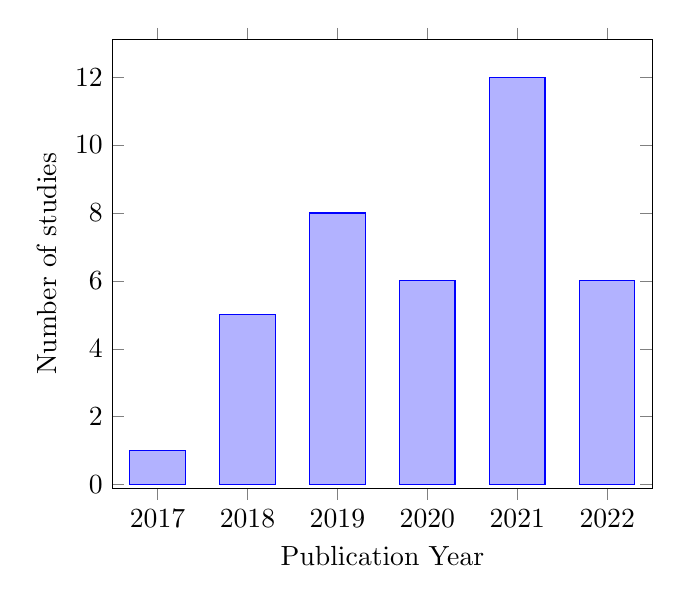
\begin{tikzpicture}
    \begin{axis}[
            ybar,
    		bar width = 20pt,
    		ylabel=Number of studies,
    		xlabel=Publication Year,
            symbolic x coords={2017,2018,2019,2020,2021,2022},
        ]
        \addplot coordinates{
    	(2017,1) (2018,5) (2019,8) (2020,6) (2021,12) (2022,6)};
    \end{axis}
	\end{tikzpicture}
	\label{fig:pubs}
\end{figure}

Furthermore, Figure~\ref{fig:pies} shows us the distribution for all reviewed paper for produce type, metric objective, detection technique used and artificial intelligence technique used. This figure presents us with evidence that suggests an overall preference of researchers towards fruits, with very few papers researching produce such as onion \cite{Nipas2022} or tomato \cite{Bautista2020-ye} \cite{Shi2019}. The overall preference towards fruits such as apple (9 papers) and mango (7 papers) leads us to believe that this representation profile of produce types is due to more apparent effects of defects and decay in fruits, which tend to change colour along their maturity process and provide a increased contrast between defects and healthy produce and facilitate the use of less precise detection techniques.

\begin{figure*}[tb]
	\centering
	\caption{Number of studies published per produce type, objective, detection technique and artificial intelligence technique}
	\resizebox{0.9\textwidth}{!}{%
	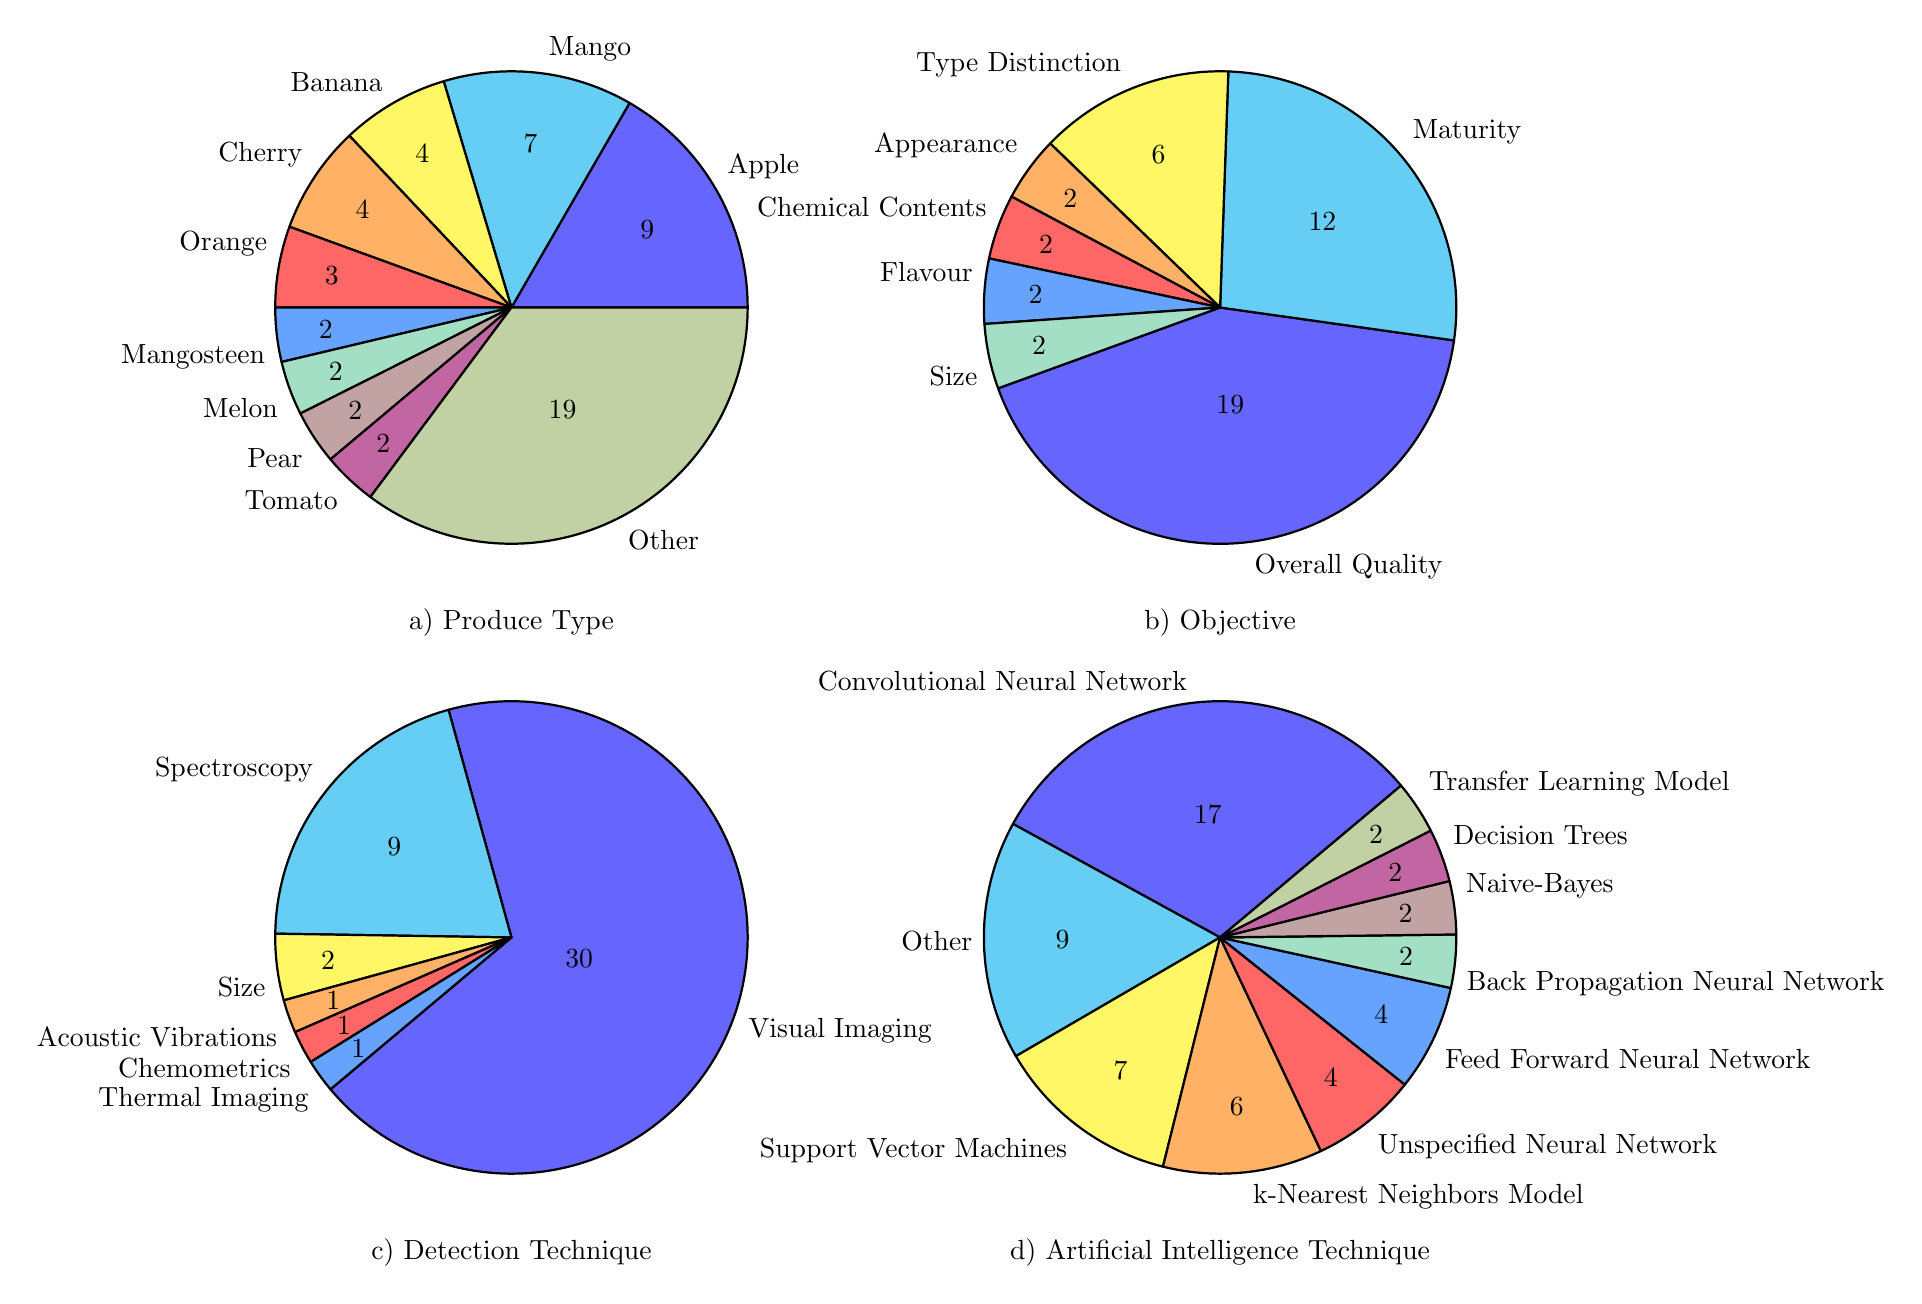
\begin{tikzpicture}
	\pie[sum=auto, pos={0,0}]{
		9/Apple,
		7/Mango,
		4/Banana,
		4/Cherry,
		3/Orange,
		2/Mangosteen,
		2/Melon,
		2/Pear,
		2/Tomato,
		19/Other
    }
	\pie[sum=auto, pos={9,0}, rotate = 200]{
		19/Overall Quality/Defect Presence,
		12/Maturity/Ripeness,
		6/Type Distinction,
		2/Appearance,
		2/Chemical Contents,
		2/Flavour,
		2/Size/Weight
    }
	\pie[sum=auto, pos={0,-8}, rotate = 220]{
		30/Visual Imaging,
		9/Spectroscopy/Spectral Imaging,
		2/Size/Weight,
		1/Acoustic Vibrations,
		1/Chemometrics,
		1/Thermal Imaging
    }
	\pie[sum=auto, pos={9,-8}, rotate = 40]{
		17/Convolutional Neural Network,
		9/Other,
		7/Support Vector Machines,
		6/k-Nearest Neighbors Model,
		4/Unspecified Neural Network,
		4/Feed Forward Neural Network,
		2/Back Propagation Neural Network,
		2/Naive-Bayes,
		2/Decision Trees,
		2/Transfer Learning Model
    }
	\node (O) at (0,-4){a) Produce Type};
	\node (O) at (9,-4){b) Objective};
	\node (O) at (0,-12){c) Detection Technique};
	\node (O) at (9,-12){d) Artificial Intelligence Technique};
	\end{tikzpicture}
	}
	\label{fig:pies}
\end{figure*}

\subsection{RQ1 - What objectives can be defined in the context of quality assessment or defect presence in produce?}

In the reviewed papers, and as can be seen in Figure~\ref{fig:pies}, 19 papers defined overall defect presence and quality detection as their objectionable metric. These papers either:

\begin{itemize}
	\item Selected defect presence as their single objective \cite{Shi2019} \cite{Annaland2020} \cite{Nipas2022} \cite{Zhang2020} \cite{Hasan2021} \cite{Azizah2017} \cite{Stasenko2021-jt}
	\item Selected defect presence as one of their quality determinator \cite{Muladi2019-jp} \cite{Nie2019-hx} \cite{Kumar2021} \cite{Choi2018-xp} \cite{Pande2019-fz} \cite{Nie2019-hx} \cite{Anita2020-nm} \cite{Park2021-de}
	\item Did not select defect presence as one of their quality determinator \cite{Pise2018} \cite{Wagimin2022} \cite{Vo2019} \cite{EAngelia2021} \cite{Bhole2020}
\end{itemize}

These objectives were extremely inline with the research question, aiming to answer to the basic question it sets.

12 papers selected maturity or ripeness of produce as their objective \cite{Hamza2018-sc} \cite{Pise2018} \cite{GarillosManliguez2021} \cite{Mohtar2019-ru} \cite{Saragih2021-wu} \cite{Mishra2022-kz} \cite{Castro2019-hk} \cite{Tamayo-Monsalve2022-ud} \cite{Prabhu2022-zh} \cite{Fadchar2020-pp} \cite{MiraeiAshtiani2021} \cite{Bhole2020}. This objective has real world importance, as ripeness and maturity can be a defining factor in produce quality and selling ability.

6 papers selected type distinction as their objective \cite{Geng2021} \cite{Zeb2022} \cite{Basri2018} \cite{Kumar2021} \cite{Pande2019-fz} \cite{Al_Haque2021-fw}. Although this objective may not present immediate usefulness in the industrialized post-harvest processes, these research endeavours pave the way for more ambidextrous systems that are interoperable between different produce types and processes.

2 papers selected appearance as their objective \cite{Choi2018-xp} \cite{Bautista2020-ye}. This goal differentiates itself from the previously mentioned quality objective, due to the author's explicit setting of this goal. As mentioned in Section~\ref{sec:intro}, certain markets prize the physical appearance of produce, increasing the market value of items deemed perfect (or close thereof). This research is then an important step in providing automated tooling for selecting these ``perfect'' examples.

2 papers selected chemical contents as their objective \cite{Lu2018} \cite{Rangel2021}. This goal was set as a stepping stone to other objectives, such as type distinction \cite{Rangel2021} and flavour profiling \cite{Lu2018}. Due to the non-destructive nature of the techniques used in both papers, this goal can be a great factor for multi-factor systems to further improve their accuracy.

2 papers selected flavour as their objective \cite{Choi2018-xp} \cite{Tran2021}. One of these papers selected specifically sweetness, a favourable quality in their target produce type, apples \cite{Tran2021}. This goal has similar usefulness as the latter papers that targeted appearance, allowing for better quality assessment and selecting ``premium'' items, as an example. The other reviewed paper included internal flavours of apples as a secondary objective towards classifying the quality of said apples \cite{Choi2018-xp}. This methodology is an example of the multi-factor systems that can be developed using other research and objectives set by researchers. 

Finally, 2 papers selected size as their objective \cite{Bautista2020-ye} \cite{Vo2019}. These systems utilized sizing as their classifying metric, mainly due to the fact that size is a preponderant factor in quality for the analysed produce: mangoes \cite{Vo2019} and tomatoes \cite{Bautista2020-ye}.

Overall, we see a variety of different objectives, with a increased number of papers aiming towards generalized goals such as quality rather than more specific ones. The review of the papers leads that this discrepancy is caused by the intrinsic uncertain nature of these generalized goals, allowing for greater flexibility when developing the presented systems.

\subsection{RQ2 - What techniques and technologies are available to analyse and monitor produce in a industrial environment?}

In the reviewed papers, and as can be seen in Figure~\ref{fig:pies}, a total of 30 papers used visual imaging techniques to analyse produce \cite{Choi2018-xp} \cite{Hamza2018-sc} \cite{Shi2019} \cite{Pise2018} \cite{GarillosManliguez2021} \cite{Annaland2020} \cite{Nipas2022} \cite{Indrabayu2019} \cite{Vo2019} \cite{Basri2018} \cite{Kumar2021} \cite{Pande2019-fz} \cite{Nie2019-hx} \cite{Bautista2020-ye} \cite{Mohtar2019-ru} \cite{Saragih2021-wu} \cite{Mishra2022-kz} \cite{Anita2020-nm} \cite{Castro2019-hk} \cite{Muladi2019-jp} \cite{Al_Haque2021-fw} \cite{Prabhu2022-zh} \cite{Park2021-de} \cite{Stasenko2021-jt} \cite{Azizah2017} \cite{Hasan2021} \cite{Zhang2020} \cite{MiraeiAshtiani2021} \cite{EAngelia2021} \cite{Bhole2020}.

While most of the reviewed papers mentioned above utilized RGB cameras, some researchers processed the resulting images further, extracting, for example, hue, saturation, value data and more from these \cite{Indrabayu2019} \cite{Castro2019-hk} or removing colour data altogether, utilizing instead boundary data to determine produce size \cite{Vo2019}. Some included other imaging system outside the visible spectrum of light, such as infra-red \cite{Annaland2020} and thermal imaging\cite{Bhole2020}. The overall preference of researchers towards these imaging systems can be explained by a variety of factors:

\begin{itemize}
	\item RGB imaging are cheap and easily available in smartphones
	\item Pre-existing datasets usually include only RGB based data points
	\item As most of the reviewed papers target fruit, RGB imaging appears to be sufficient to detect changes in the skin of said fruit.
\end{itemize}

9 papers utilized spectroscopy or spectral imaging to analyse produce. Of these:

\begin{itemize}
	\item 2 used unspecified spectral band spectroscopy \cite{Geng2021} \cite{GarillosManliguez2021}
	\item 7 used near-infrared spectroscopy \cite{Zeb2022} \cite{Tran2021} \cite{Annaland2020} \cite{Lu2018} \cite{Choi2018-xp} \cite{Tamayo-Monsalve2022-ud} \cite{Rangel2021}
\end{itemize}

Spectral imaging appears to be a promising technique to develop detection systems, due to the different abilities it provides based on the spectral band measured. Depending on these, systems are able to detect surface or internal defects and features \cite{Geng2021}. However, the cost of these systems as well as the research required to select the appropriate spectral bands may prove a bottleneck for this technique.

2 papers utilized size in their systems \cite{Choi2018-xp} \cite{Wagimin2022}. Both papers utilize size as a basis for quality detection, due to its prominent effect on grading for the analysed produce: pears \cite{Choi2018-xp} and Mangoes \cite{Wagimin2022}.

Finally, 3 papers utilized acoustic vibrations \cite{Fadchar2020-pp}, chemometrics \cite{Rangel2021} and thermal imaging \cite{Bhole2020}. One of the papers used the sound signatures of dropping coconuts in water to detect their ripeness. This technique, although interesting, may provide little real world value due to its impracticality. One paper utilized chemometrics to relate near infrared spectroscopy to chemical content in watermelons \cite{Rangel2021}. This technique can be useful when utilized with non-destructive detection systems that provide data regarding chemical content. Finally, one paper utilized thermal imaging and RGB imaging to grade mangoes \cite{Bhole2020}. This system provides an interesting detection system, however, different environments may provide obstacles to proper temperature detection and analysis using these systems.

Overall, it can be ascertained that although there is variety in detection systems used by the reviewed papers, there is a tendency towards less complex and more available systems for detection such as RGB cameras.

\subsection{RQ3 - What techniques and technologies previously researched utilize artificial intelligence, and how?}

In the reviewed papers, and as can be seen in Figure~\ref{fig:pies}, a total of 29 papers utilized neural networks as their artificial intelligence technique. Of these:

\begin{itemize}
	\item 17 used convolutional neural networks \cite{Pande2019-fz} \cite{Mohtar2019-ru} \cite{Saragih2021-wu} \cite{Al_Haque2021-fw} \cite{Tamayo-Monsalve2022-ud} \cite{Park2021-de} \cite{Stasenko2021-jt} \cite{Azizah2017} \cite{Hasan2021} \cite{MiraeiAshtiani2021} \cite{Basri2018} \cite{Kumar2021} \cite{GarillosManliguez2021} \cite{Shi2019} \cite{EAngelia2021} \cite{Bhole2020} \cite{Geng2021}
	\item 4 used neural networks of unspecified architecture \cite{Fadchar2020-pp} \cite{Anita2020-nm} \cite{Wagimin2022} \cite{Castro2019-hk}
	\item 4 used feed forward neural networks \cite{Choi2018-xp} \cite{Hamza2018-sc} \cite{Bautista2020-ye} \cite{Rangel2021}
	\item 2 used back propagation neural networks \cite{Nie2019-hx}, \cite{Muladi2019-jp}
	\item 1 used convolutional Siamese neural networks \cite{Annaland2020}
	\item 1 used an extreme learning model \cite{Lu2018}
\end{itemize}

This overwhelming majority of researchers choosing to use neural networks in their research can be attributed to some factors:

\begin{itemize}
	\item Neural Networks are currently one of the easier machine learning models to implement, using tools such as Keras\footnote{\url{https://keras.io/}}
	\item Most of the used datasets are of images and neural networks are more established in that data space
	\item Automated training of these networks provides an easier process for researchers that are not focused on the artificial intelligence component of their systems
\end{itemize}

7 papers utilised support vector machines \cite{Zeb2022} \cite{Tran2021} \cite{Indrabayu2019} \cite{Castro2019-hk} \cite{Prabhu2022-zh} \cite{Vo2019} \cite{Wagimin2022}. One of these compared support vector machines, an unspecified neural network and a k-Nearest Neighbors model at the task of grading mangoes \cite{Wagimin2022}, with the support vector machine model being the most accurate model.

One paper compared support vector machines and Naive-Bayes in the task of grading mangoes \cite{Pise2018}. The researchers found that Naive-Bayes was slightly faster at grading mangoes than a support vector machine model.

One paper compared support vector machines, k-Nearest Neighbors, a multiple linear regression model and a discriminant analysis model in the task of classifying apples based on sweetness \cite{Tran2021}. The researchers found that the discriminant analysis model was the best performing model.

One paper compared several techniques, including Decision Trees, Naive-Bayes, Support Vector Machines, k-Nearest Neighbors and an unspecified neural network at distinguishing between fruits using spectroscopy data \cite{Zeb2022}. The authors found comparatively similar accuracy results for all evaluated models.

One paper compared several techniques, including Principal Component Regression, Partial Least Squares and Feed Forward Neural Network, to predict chemical components from spectroscopy data \cite{Rangel2021}.

Overall, the review revealed that in this specific subdomain, researchers undertake their more relevant work on the detection systems themselves rather than the artificial intelligence componentry, using said components as commodities rather than focus of study. As such, most if not all papers reviewed select some models, compare them and select the one deemed most competent. This does not create meaningful advances for artificial intelligence, but does demonstrate the ubiquity of artificial intelligence usage.

\section{Conclusion and future work}
\label{sec:conc}

This work presents a systematic review in the topic of quality assessment and defect detection in produce. Of the 366 initially retrieved studies, 86 were approved for full-text reading and 38 were included in this review. These studies responded to 3 research questions regarding target produce type, detection systems and artificial intelligence usage. The research throughput throughout the last 5 years has remained steady.

From the review process it was possible to determine that researchers are generally more interested on analysing fruits rather than vegetables, with the vast majority of papers targeting fruits. Furthermore, fruits with colour changes based on ripeness and decay were also more selected (such as apples, bananas and mangoes). The studies also targeted different stages of the agricultural process, from growing, harvest and post-harvest specificity. Further research problems are available, with plenty of produce types, such as potatoes, available to study and investigate.

Most reviewed papers also specified objectives for their investigation based on maturity and overall quality. The latter also regularly included defect detection as part of it's system. This fulfils the topic statement quite well, attempting to directly assess the quality of the produce at hand. However, more research can be executed on firmly determining causational relationships between secondary objectives such as chemical contents and the overall quality.

Most papers utilized computer vision systems to monitor the produce at hand. This cheap, accessible solution is extremely well suited for industrial environments, such as automated facilities. However, other detection techniques have shown good results, such has spectral based approaches (e.g., multi spectral imaging and spectroscopy). Furthermore, research can still be done on multi-modal detection systems, which utilize more than 1 type of sensor to further improve their results.

Finally, the executed review ascertained that most if not all papers included do not provide innovative utilization of artificial intelligence methods in the field, but rather utilize commoditized versions to handle the gathered data. As such, research is still plentifully available, with regards to new and improved artificial intelligence systems as well as domain specific models.

Overall, the quality assessment and defect detection topic in the agricultural and artificial intelligence field produces good research, with multiple target produce types, methods and objectives. As for future work, the limited existence of multi-target systems that target both fruit and vegetables provides a great opportunity for further research by the authors.

\bibliographystyle{IEEEtranN}
\bibliography{references/introduction,references/method,references/results}

\end{document}